\documentclass[landscape,a3paper]{article}
\usepackage[margin=0.5in]{geometry}
\usepackage{tikz}
\usetikzlibrary{shapes.multipart, positioning, arrows.meta, calc, fit, backgrounds}
\usepackage{xcolor}

\definecolor{entityColor}{RGB}{52, 152, 219}
\definecolor{junctionColor}{RGB}{241, 196, 15}
\definecolor{pkColor}{RGB}{231, 76, 60}
\definecolor{fkColor}{RGB}{46, 204, 113}

\tikzset{
    entity/.style={
        rectangle split,
        rectangle split parts=2,
        draw=entityColor,
        very thick,
        fill=entityColor!10,
        text width=3cm,
        align=center,
        rounded corners=3pt
    },
    junction/.style={
        rectangle split,
        rectangle split parts=2,
        draw=junctionColor,
        very thick,
        fill=junctionColor!10,
        text width=2.8cm,
        align=center,
        rounded corners=3pt
    },
    relationship/.style={
        ->,
        >=Stealth,
        very thick,
        draw=gray!70
    },
    manytomany/.style={
        <->,
        >=Stealth,
        very thick,
        draw=gray!70,
        dashed
    },
    label/.style={
        font=\small,
        text=black
    }
}

\begin{document}

\begin{titlepage}
\centering
\vspace*{2cm}
{\Huge\bfseries SavoyConnect\\[0.5cm] Eagle Level ER Diagram\par}
\vspace{1cm}
{\Large 7 Core Entities with Relationships\par}
\vspace{2cm}
{\large November 19, 2025\par}
\vfill
{\large Database Design Document\par}
\end{titlepage}

\newpage

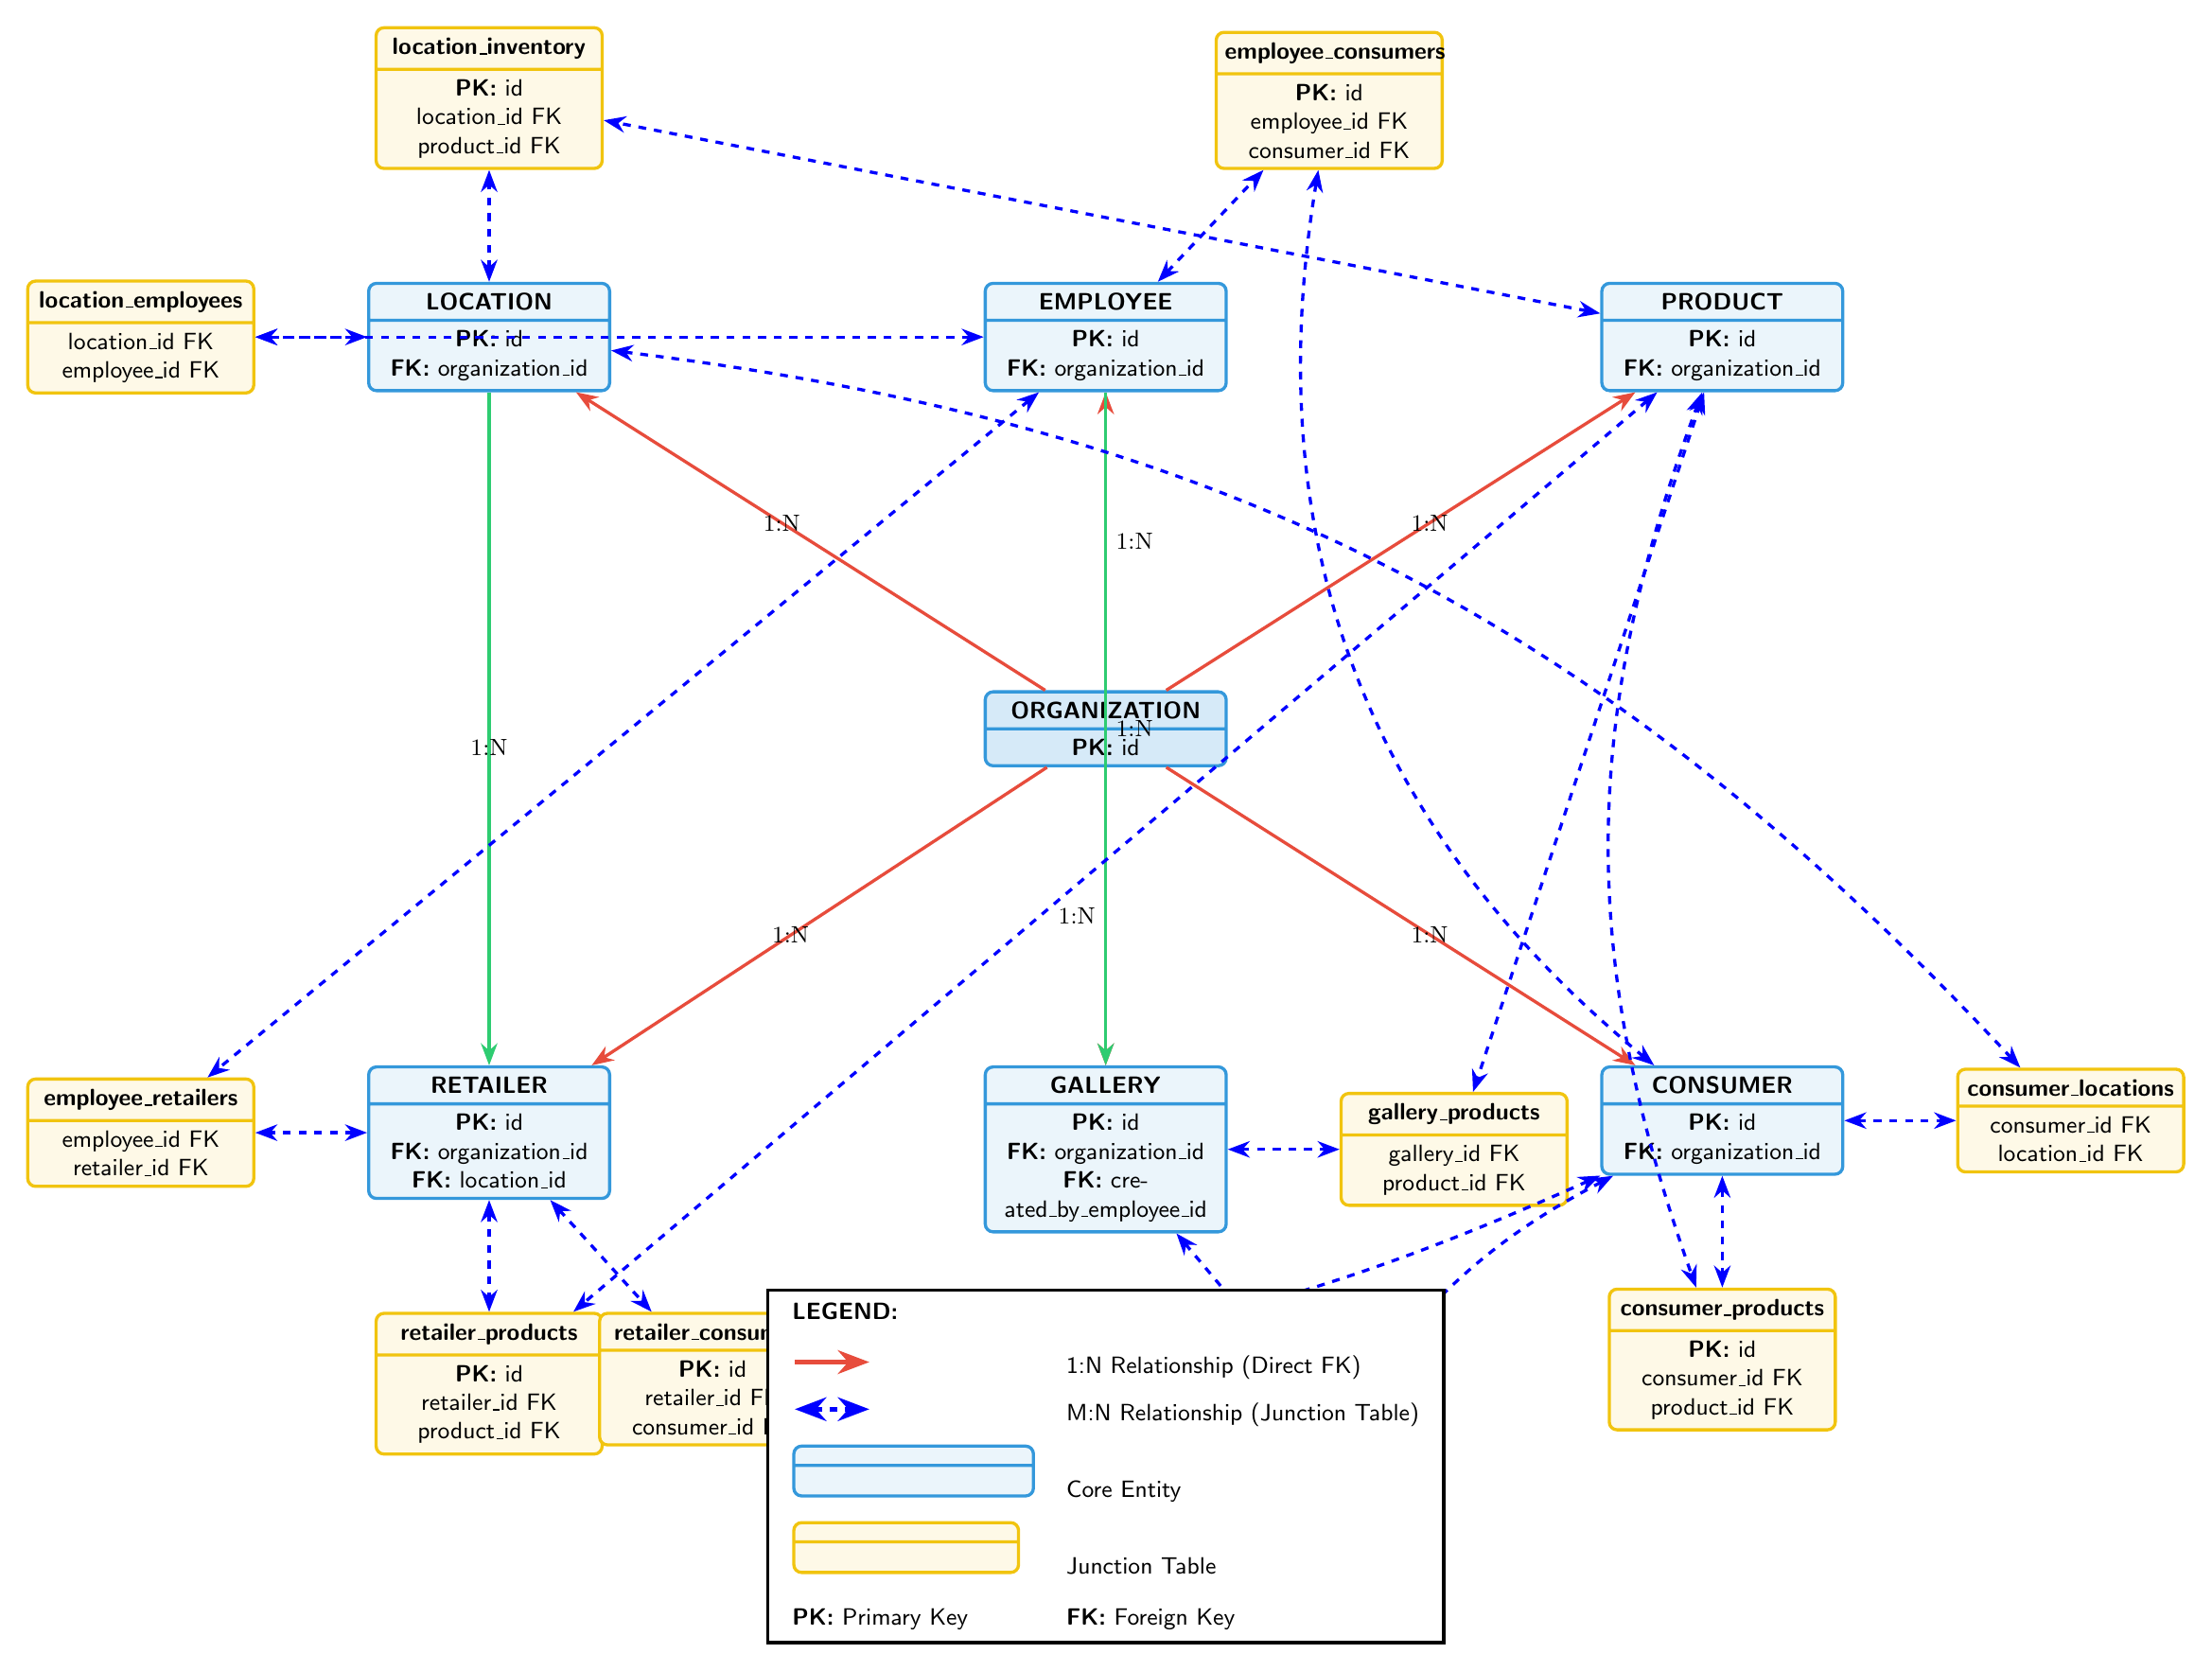
\begin{tikzpicture}[node distance=4cm and 5cm, every node/.style={font=\small\sffamily}]

    % ============================================
    % CORE ENTITIES
    % ============================================
    
    % ORGANIZATION (Center)
    \node[entity, fill=entityColor!20] (org) {
        \textbf{ORGANIZATION}
        \nodepart{second}
        \textbf{PK:} id
    };
    
    % LOCATION (Top Left)
    \node[entity, above left=of org] (loc) {
        \textbf{LOCATION}
        \nodepart{second}
        \textbf{PK:} id\\
        \textbf{FK:} organization\_id
    };
    
    % EMPLOYEE (Top)
    \node[entity, above=of org] (emp) {
        \textbf{EMPLOYEE}
        \nodepart{second}
        \textbf{PK:} id\\
        \textbf{FK:} organization\_id
    };
    
    % PRODUCT (Top Right)
    \node[entity, above right=of org] (prod) {
        \textbf{PRODUCT}
        \nodepart{second}
        \textbf{PK:} id\\
        \textbf{FK:} organization\_id
    };
    
    % RETAILER (Bottom Left)
    \node[entity, below left=of org] (ret) {
        \textbf{RETAILER}
        \nodepart{second}
        \textbf{PK:} id\\
        \textbf{FK:} organization\_id\\
        \textbf{FK:} location\_id
    };
    
    % GALLERY (Bottom)
    \node[entity, below=of org] (gal) {
        \textbf{GALLERY}
        \nodepart{second}
        \textbf{PK:} id\\
        \textbf{FK:} organization\_id\\
        \textbf{FK:} created\_by\_employee\_id
    };
    
    % CONSUMER (Bottom Right)
    \node[entity, below right=of org] (con) {
        \textbf{CONSUMER}
        \nodepart{second}
        \textbf{PK:} id\\
        \textbf{FK:} organization\_id
    };
    
    % ============================================
    % JUNCTION TABLES (Around the edges)
    % ============================================
    
    % Location-Employee Junction
    \node[junction, left=1.5cm of loc] (loc_emp) {
        \textbf{location\_employees}
        \nodepart{second}
        location\_id FK\\
        employee\_id FK
    };
    
    % Location-Inventory Junction
    \node[junction, above=1.5cm of loc] (loc_inv) {
        \textbf{location\_inventory}
        \nodepart{second}
        \textbf{PK:} id\\
        location\_id FK\\
        product\_id FK
    };
    
    % Employee-Retailer Junction
    \node[junction, left=1.5cm of ret] (emp_ret) {
        \textbf{employee\_retailers}
        \nodepart{second}
        employee\_id FK\\
        retailer\_id FK
    };
    
    % Retailer-Products Junction
    \node[junction, below=1.5cm of ret] (ret_prod) {
        \textbf{retailer\_products}
        \nodepart{second}
        \textbf{PK:} id\\
        retailer\_id FK\\
        product\_id FK
    };
    
    % Gallery-Products Junction
    \node[junction, right=1.5cm of gal] (gal_prod) {
        \textbf{gallery\_products}
        \nodepart{second}
        gallery\_id FK\\
        product\_id FK
    };
    
    % Consumer-Locations Junction
    \node[junction, right=1.5cm of con] (con_loc) {
        \textbf{consumer\_locations}
        \nodepart{second}
        consumer\_id FK\\
        location\_id FK
    };
    
    % Consumer-Products Junction
    \node[junction, below=1.5cm of con] (con_prod) {
        \textbf{consumer\_products}
        \nodepart{second}
        \textbf{PK:} id\\
        consumer\_id FK\\
        product\_id FK
    };
    
    % Retailer-Consumers Junction
    \node[junction, below=1.5cm of ret, xshift=3cm] (ret_con) {
        \textbf{retailer\_consumers}
        \nodepart{second}
        \textbf{PK:} id\\
        retailer\_id FK\\
        consumer\_id FK
    };
    
    % Gallery-Views Junction
    \node[junction, below=1.5cm of gal, xshift=3cm] (gal_view) {
        \textbf{gallery\_views}
        \nodepart{second}
        \textbf{PK:} id\\
        gallery\_id FK\\
        consumer\_id FK
    };
    
    % Employee-Consumers Junction
    \node[junction, above=1.5cm of emp, xshift=3cm] (emp_con) {
        \textbf{employee\_consumers}
        \nodepart{second}
        \textbf{PK:} id\\
        employee\_id FK\\
        consumer\_id FK
    };
    
    % ============================================
    % RELATIONSHIPS (1:N - Direct FK)
    % ============================================
    
    % ORGANIZATION to all entities (1:N)
    \draw[relationship, pkColor] (org) -- node[label, above left] {1:N} (loc);
    \draw[relationship, pkColor] (org) -- node[label, right] {1:N} (emp);
    \draw[relationship, pkColor] (org) -- node[label, above right] {1:N} (prod);
    \draw[relationship, pkColor] (org) -- node[label, below left] {1:N} (ret);
    \draw[relationship, pkColor] (org) -- node[label, left] {1:N} (gal);
    \draw[relationship, pkColor] (org) -- node[label, below right] {1:N} (con);
    
    % LOCATION to RETAILER (1:N)
    \draw[relationship, fkColor] (loc) -- node[label, below] {1:N} (ret);
    
    % EMPLOYEE to GALLERY (1:N)
    \draw[relationship, fkColor] (emp) -- node[label, right] {1:N} (gal);
    
    % ============================================
    % M:N RELATIONSHIPS (via Junction Tables)
    % ============================================
    
    % Location-Employee M:N
    \draw[manytomany, blue] (loc) -- (loc_emp);
    \draw[manytomany, blue] (emp) -- (loc_emp);
    
    % Location-Product M:N (Inventory)
    \draw[manytomany, blue] (loc) -- (loc_inv);
    \draw[manytomany, blue] (prod) -- (loc_inv);
    
    % Employee-Retailer M:N
    \draw[manytomany, blue] (emp) -- (emp_ret);
    \draw[manytomany, blue] (ret) -- (emp_ret);
    
    % Retailer-Product M:N
    \draw[manytomany, blue] (ret) -- (ret_prod);
    \draw[manytomany, blue] (prod) -- (ret_prod);
    
    % Gallery-Product M:N
    \draw[manytomany, blue] (gal) -- (gal_prod);
    \draw[manytomany, blue] (prod) -- (gal_prod);
    
    % Consumer-Location M:N
    \draw[manytomany, blue] (con) -- (con_loc);
    \draw[manytomany, blue] (loc) to[bend left=20] (con_loc);
    
    % Consumer-Product M:N
    \draw[manytomany, blue] (con) -- (con_prod);
    \draw[manytomany, blue] (prod) to[bend right=20] (con_prod);
    
    % Retailer-Consumer M:N
    \draw[manytomany, blue] (ret) -- (ret_con);
    \draw[manytomany, blue] (con) to[bend left=10] (ret_con);
    
    % Gallery-Consumer M:N
    \draw[manytomany, blue] (gal) -- (gal_view);
    \draw[manytomany, blue] (con) to[bend right=10] (gal_view);
    
    % Employee-Consumer M:N
    \draw[manytomany, blue] (emp) -- (emp_con);
    \draw[manytomany, blue] (con) to[bend left=30] (emp_con);
    
    % ============================================
    % LEGEND
    % ============================================
    
    \node[draw, rectangle, very thick, fill=white, below=7cm of org] (legend) {
        \begin{tabular}{ll}
        \textbf{LEGEND:} & \\[0.3cm]
        \tikz\draw[relationship, pkColor, line width=2pt] (0,0) -- (1,0); & 1:N Relationship (Direct FK) \\[0.2cm]
        \tikz\draw[manytomany, blue, line width=2pt] (0,0) -- (1,0); & M:N Relationship (Junction Table) \\[0.2cm]
        \tikz\node[entity, minimum width=2cm] {}; & Core Entity \\[0.2cm]
        \tikz\node[junction, minimum width=2cm] {}; & Junction Table \\[0.3cm]
        \textbf{PK:} Primary Key & \textbf{FK:} Foreign Key \\
        \end{tabular}
    };
    
\end{tikzpicture}

\newpage

% ============================================
% RELATIONSHIP SUMMARY PAGE
% ============================================

\section*{Relationship Summary}

\subsection*{1:N Relationships (Direct Foreign Keys)}

\begin{enumerate}
    \item \textbf{ORGANIZATION $\rightarrow$ LOCATION} (1:N)\\
    One organization owns many locations
    
    \item \textbf{ORGANIZATION $\rightarrow$ EMPLOYEE} (1:N)\\
    One organization employs many employees
    
    \item \textbf{ORGANIZATION $\rightarrow$ PRODUCT} (1:N)\\
    One organization manufactures many products
    
    \item \textbf{ORGANIZATION $\rightarrow$ RETAILER} (1:N)\\
    One organization partners with many retailers
    
    \item \textbf{ORGANIZATION $\rightarrow$ GALLERY} (1:N)\\
    One organization owns many gallery items
    
    \item \textbf{ORGANIZATION $\rightarrow$ CONSUMER} (1:N)\\
    One organization serves many consumers
    
    \item \textbf{LOCATION $\rightarrow$ RETAILER} (1:N)\\
    One location supplies many retailers
    
    \item \textbf{EMPLOYEE $\rightarrow$ GALLERY} (1:N)\\
    One employee creates many gallery items
\end{enumerate}

\subsection*{M:N Relationships (Junction Tables)}

\begin{enumerate}
    \item \textbf{LOCATION $\leftrightarrow$ EMPLOYEE} via \texttt{location\_employees}\\
    Employees work at multiple locations
    
    \item \textbf{LOCATION $\leftrightarrow$ PRODUCT} via \texttt{location\_inventory}\\
    Locations stock multiple products with quantities
    
    \item \textbf{EMPLOYEE $\leftrightarrow$ RETAILER} via \texttt{employee\_retailers}\\
    Sales reps manage multiple retailer accounts
    
    \item \textbf{RETAILER $\leftrightarrow$ PRODUCT} via \texttt{retailer\_products}\\
    Retailers sell multiple products
    
    \item \textbf{GALLERY $\leftrightarrow$ PRODUCT} via \texttt{gallery\_products}\\
    Gallery items showcase multiple products
    
    \item \textbf{CONSUMER $\leftrightarrow$ LOCATION} via \texttt{consumer\_locations}\\
    Consumers order from multiple locations
    
    \item \textbf{CONSUMER $\leftrightarrow$ PRODUCT} via \texttt{consumer\_products}\\
    Consumers purchase multiple products
    
    \item \textbf{RETAILER $\leftrightarrow$ CONSUMER} via \texttt{retailer\_consumers}\\
    Retailers serve multiple consumers
    
    \item \textbf{GALLERY $\leftrightarrow$ CONSUMER} via \texttt{gallery\_views}\\
    Consumers view multiple gallery items
    
    \item \textbf{EMPLOYEE $\leftrightarrow$ CONSUMER} via \texttt{employee\_consumers}\\
    Employees serve multiple consumers
\end{enumerate}

\vfill

\begin{center}
\fbox{\parbox{0.8\textwidth}{
\textbf{Total Tables:} 17 (7 Core Entities + 10 Junction Tables)\\
\textbf{Total Relationships:} 18 (8 Direct FK + 10 M:N)\\
\textbf{Normalization:} Third Normal Form (3NF)\\
\textbf{Multi-tenant:} Yes (via organization\_id)
}}
\end{center}

\end{document}
